\RequirePackage{amsmath}
\documentclass[runningheads]{llncs}
%
\usepackage[T1]{fontenc}
\usepackage{float}
\usepackage{graphicx}
\usepackage{subcaption}
\usepackage[inline]{enumitem}
% Used for displaying a sample figure. If possible, figure files should
% be included in EPS format.
%
% If you use the hyperref package, please uncomment the following two lines
% to display URLs in blue roman font according to Springer's eBook style:
%\usepackage{color}
%\renewcommand\UrlFont{\color{blue}\rmfamily}
%\urlstyle{rm}

\usepackage{tikz} 
\usetikzlibrary{
    calc,
    decorations.pathmorphing,
    decorations.pathreplacing, 
    shapes.geometric, 
} 

\usepackage{macros}
\usepackage[capitalise,noabbrev]{cleveref}

\begin{document}
%
\title{Realizing Graphs with Cut Constraints}
% Tikz
%\titlerunning{Abbreviated paper title}
% If the paper title is too long for the running head, you can set
% an abbreviated paper title here
%

\author{
Vítor Gomes Chagas\inst{1}\orcidID{0000-0002-6506-4174}
\and \\
Samuel Plaça de Paula\inst{1}\orcidID{0009-0005-5970-2984}
\and \\
Greis Yvet Oropeza Quesquén\inst{1}\orcidID{0000-0003-0112-8009}
\and \\
Lucas de Oliveira Silva\inst{1}\orcidID{0000-0002-7846-5903}
\and \\
Uéverton dos Santos Souza\inst{2,3}\orcidID{0000-0002-5320-9209}
}

\authorrunning{V. G. Chagas et al.}
% First names are abbreviated in the running head.
% If there are more than two authors, 'et al.' is used.
%

\institute{
Instituto de Computação, Universidade Estadual de Campinas, Campinas, Brazil\\
\email{vitor.chagas@ic.unicamp.br} \\
\email{s233554@dac.unicamp.br} \\
\email{greis.quesquen@ic.unicamp.br} \\
\email{lucas.oliveira.silva@ic.unicamp.br} \\
\and
IMPA, Instituto de Matemática Pura e Aplicada, Rio de Janeiro, Brazil\\
\and
Instituto de Computação, Universidade Federal Fluminense, Niterói, Brazil\\
\email{ueverton.souza@impatech.org.br}}

%
\maketitle % typeset the header of the contribution
%
\begin{abstract}
%The abstract should briefly summarize the contents of the paper in 150--250 words.

Given a finite non-decreasing sequence $\texttt{d}=(d_1,\ldots,d_n)$ of natural numbers, % such that $d_1\geq d_2 \geq \ldots \geq d_n$, 
the \GRfull~problem asks whether \texttt{d} is a graphic sequence, i.e., there exists a labeled simple graph such that $(d_1,\ldots,d_n)$ is the degree sequence of this graph. Such a problem can be solved in polynomial time due to the Erd\H{o}s and Gallai characterization of graphic sequences. 
%In particular, \texttt{d} is graphic if and only if $\sum\limits_{i=1}^n d_i$ is even and $\sum\limits_{i=1}^k d_k \leq k(k-1) + \sum\limits_{j=k+1}^n\min\{k,d_j\}$ for all $k\in\{1,\ldots,n\}$.
Since vertex degree is the size of a trivial edge cut, we consider a natural generalization of \GRfull, where we are given a finite sequence $\texttt{d}=(d_1,\ldots,d_n)$ of natural numbers (representing the trivial edge cut sizes) and a list of nontrivial cut constraints $\call$ composed of pairs $(S_j,\ell_j)$ where $S_j\subset \{v_1,\ldots,v_n\}$, and $\ell_j$ is a natural number.
%
In such a problem, we are asked whether there is a simple graph with vertex set $V=\{v_1,\ldots,v_n\}$ such that $v_i$ has degree $d_i$ and $\partial(S_j)$ is an edge cut of size $\ell_j$, for each $(S_j,\ell_j)\in \call$. We show that such a problem is polynomial-time solvable whenever each $S_j$ has size at most three. Conversely, assuming P~$\neq$~NP, we prove that it cannot be solved in polynomial time when $\call$ contains pairs with sets of size four, and our hardness result holds even assuming that each $d_i$ of \texttt{d} equals $1$. 

\keywords{Graph realization \and Degree sequence \and Graph factor}
\end{abstract}
%
%
%
% guidelines do CIAC deteminam que a página de título contenha só até o abstract
\newpage

\section{Introduction}

% State of the world (robots for creative activites)
The term ``robot,'' originally signifying `forced labor,' has long been associated with labor and work. Robots have demonstrated their utility in various automated productive and social contexts, where the primary goals are improving productivity, safety, and fostering social interactions with humans~\cite{simoes2022designing, weidemann2021role, honig2018understanding}. However, an increasing number of cases feature using of robots in creative settings. Unlike productive contexts, where the focus is on efficiency and task completion~\cite{arents2022smart}, or social contexts, where communication and trust are prioritized~\cite{nam2020trust, saunderson2019robots}, creative environments prioritize artistic innovation and expression~\cite{hsueh2024counts}. This shift fundamentally alters the dynamics of human-robot interaction, redefining the roles and expectations for both humans and robots.

For instance, robots’ social behaviors are leveraged to support the generation and expression of creative ideas~\cite{hu2021exploring, sandoval2022human, alves2020creativity}, and programmable robotic movements and trajectories are employed to inspire artistic activities such as sketching~\cite{lin2020your}. These studies often engage participants from creative fields who possess limited prior experience with robotics, and are typically conducted in short-term, experimental settings. Consequently, the findings from these studies remain constrained since much can be learned from professional practitioners' experiences to inform system design such as digital fabrication~\cite{hirsch2023nothing}. There is a notable gap in research examining the long-term, active, and practical experience of integrating robotic systems into the creative processes. As a result, the deeper insights into how robots facilitate and shape creative processes, beyond simply augmenting human creativity, remain underexplored. In this study, we aim to better understand the impacts of robots on creative processes and outcomes.

As early as Leonardo da Vinci's 16th century ``Automaton,'' artists have explored the creative affordances of robotic systems~\cite{shanken2002cybernetics, pagliarini2009development, jeon2017robotic}. The artistic creation process typically encompasses various stages, including the exploration of materials and techniques, ongoing experimentation and iteration, and the continual refinement of the artists' insights into their creative subjects~\cite{lewis2023art, sturdee2022state}. Therefore, investigating the artistic process involving robots offers an opportunity to gain deeper insights into robots' creative potential. Robotic art, in particular, provides a compelling case for this exploration.

We define robotic art as artworks that utilize robotic or automated machines to create artistic experiences and tangible artifacts. One example is robotic installation art, in which robots are programmed to follow specific rules that embody the artist’s expression (\autoref{fig:teaser} (a)). Another example is responsive art, in which robots react to their environment, with behaviors that change over time or in response to spectators (\autoref{fig:teaser} (b)). Additionally, there are robotic creators, which possess a degree of agency, allowing them to collaborate with human artists and produce works that extend beyond mere replication of human-created art (\autoref{fig:teaser} (c) and (d)). As such, robotic art becomes a rich case for exploring human-machine interactions in creative contexts. Gaining a deeper understanding of how robots facilitate artistic expression can provide insights for designing computing systems to support creative activities~\cite{gomez2021robot}.

% Therefore, we did...
We draw on semi-structured, in-depth interviews with renowned professional robotic artists to investigate the use of robots in artistic practice. Specifically, our goal is to understand how artistic exploration of robotic systems challenges conventional assumptions about the functions of robots, such as their roles in automating repetitive tasks or serving human needs. We also explore the implications of robots in the artistic process and examine how creativity may emerge within robotic art. To address these interrelated inquiries, our study focuses on the practice of robotic art, posing the research question: \textit{How do robotic artists utilize robots in their artistic practice?} We approach this inquiry through the perspectives and experiences of robotic artists, who creatively design, modify, and repurpose robotic systems for artistic expression and exploration.

% The key findings are...
Our findings highlight the social, material, and temporal dimensions of artists' practices that shape their creativity and artistic outcomes. The creation of robotic art is largely a social process, as artists receive both explicit and implicit feedback through the audience's reactions and reception of their work. Simultaneously, the embodiment and malfunctions inherent to robotic systems drive artistic experimentation. The temporal processes of creation and exhibition, beyond just the final product, further enhance the creative value. Our empirical analysis presents how creativity emerges through the interplay of social, material, and temporal interactions among artists, robots, audiences, and the environment.

% The contributions of this work are...
We make two main contributions to HCI in this study. 
First, we elucidate the interactive mechanisms among key actors---human creators, machines, audiences, and environments---within the practice of robotic art, a topic that remains underexplored in HCI. Our findings reveal the significance of sociality (e.g., interactions between artists and audiences), materiality (e.g., the embodiment and malfunctions of robots), and temporality (e.g., the processes of creation and exhibition) in shaping creative values. We propose that these three facets are central to the creative process and facilitate the emergence of creativity in robotic art.
Second, drawing from the findings, we offer implications for \textit{socially informed}, \textit{material-attentive}, and \textit{process-oriented} creation with computing systems. We suggest leveraging these three aspects to enhance creativity and the creative experience. Specifically, we discuss the value of incorporating implicit audience feedback, designing with technical malfunctions, and focusing on the post-creation process to foster alternative creative experiences with machines~\cite{alter2010designing, juarez2022glitch}.



% \newpage

\section{Preliminaries}
\label{sec:sec-Preliminary}




\begin{table}[t]
  \caption{
  Space complexity of various approximate matrix multiplication algorithms in the sliding-window setting. 
  %Note that the final complexity is scaled by \(O(d_x + d_y)\).
  %Space complexity for various AMM algorithms under the sliding-window setting.
  }
  \vspace{-2mm}
  \label{tab:table-comparsion}
  \renewcommand{\arraystretch}{1.5}
  \begin{tabular}{|c|c|c|}
    \hline
    Algorithm & Normalized model & Unnormalized model \\
    \hline
    Sampling \cite{efraimidis2006weighted, drineas2006fast,babcock2001sampling} & $O(\frac{d_x + d_y}{\epsilon^2}\log{N})$ & $O\left(\frac{d_x + d_y}{\epsilon^2}\log{NR}\right)$ \\
    \hline
    DI-COD \cite{YaoLCWC24} & $O(\frac{d_x + d_y}{\epsilon}\log^2{\frac{1}{\epsilon}})$ & $O\left(\frac{(d_x + d_y)\cdot R}{\epsilon}\log^2{\frac{R}{\epsilon}}\right)$\\
    \hline
    EH-COD \cite{YaoLCWC24} & $O(\frac{d_x + d_y}{\epsilon^2}\log{\epsilon N})$ & $O\left(\frac{d_x + d_y}{\epsilon^2}\log{\epsilon NR}\right)$ \\
    \hline
    % DI-SCOD \cite{YaoLCWC24} & $O(\frac{d_x + d_y}{\epsilon}\log^2{\frac{1}{\epsilon}})$ & $O\left(\frac{(d_x + d_y)\cdot R}{\epsilon}\log^2{\frac{R}{\epsilon}}\right)$\\
    % \hline
    % EH-SCOD \cite{YaoLCWC24} & $O(\frac{d_x + d_y}{\epsilon^2})$ & $O\left(\frac{d_x + d_y}{\epsilon^2}\log{R}\right)$ \\
    % \hline
    {\oursolution} (Ours) & $O(\frac{d_x + d_y}{\epsilon})$ & $O\left(\frac{d_x + d_y}{\epsilon}\log{R}\right)$ \\
    \hline
\end{tabular}
\vspace{-1mm}
\end{table}

\subsection{Notations and Basic Concepts}

In this paper, we use bold uppercase letters to denote matrices (e.g., $\boldsymbol{A}$), bold lowercase letters to denote vectors (e.g., $\boldsymbol{x}$), and lowercase letters to denote scalars (e.g., $w$).


Given a real matrix \(\boldsymbol{A} \in \mathbb{R}^{n\times m}\), its condensed singular value decomposition (SVD) is given by \(\boldsymbol{A} = \boldsymbol{U} \boldsymbol{\Sigma} \boldsymbol{V}^\top\), where \(\boldsymbol{U} \in \mathbb{R}^{n \times r}\) and \(\boldsymbol{V} \in \mathbb{R}^{m \times r}\) are matrices with orthonormal columns, and \(\boldsymbol{\Sigma} = \operatorname{diag}(\sigma_1, \sigma_2, \dots, \sigma_r)\) is a diagonal matrix containing the singular values of \(\boldsymbol{A}\) arranged in non-increasing order, i.e., \(\sigma_1 \geq \sigma_2 \geq \cdots \geq \sigma_r > 0\), with \(r\) denoting the rank of \(\boldsymbol{A}\). We define several matrix norms as follows: the Frobenius norm of \(\boldsymbol{A}\) is given by 
\(
\|\boldsymbol{A}\|_F = \sqrt{\sum_{i,j} A_{i,j}^2} = \sqrt{\sum_{i=1}^r \sigma_i^2},
\)
the spectral norm is 
\(
\|\boldsymbol{A}\|_2 = \sigma_1,
\)
and the nuclear norm is 
\(
\|\boldsymbol{A}\|_* = \sum_{i=1}^r \sigma_i.
\)
For a matrix \(\boldsymbol{A}\), we denote its \(i\)-th column by \(\boldsymbol{a}_i\); hence, if \(\boldsymbol{A} \in \mathbb{R}^{n \times l}\) and \(\boldsymbol{B} \in \mathbb{R}^{m \times l}\), then their product can be expressed as: 
\(
\boldsymbol{A}\boldsymbol{B}^T = \sum_{i=1}^l \boldsymbol{a}_i \boldsymbol{b}_i^T.
\)
Finally, \(\boldsymbol{I}_n\) denotes the \(n \times n\) identity matrix and \(\boldsymbol{0}^{n \times m}\) denotes the \(n \times m\) zero matrix.








\subsection{Problem Definition}
The Approximate Matrix Multiplication (AMM) problem has been extensively studied in the literature \cite{YeLZ16,MrouehMG17,drineas2006fast,FrancisR22}. Given two matrices \(\boldsymbol{X} \in \mathbb{R}^{d_x \times n}\) and \(\boldsymbol{Y} \in \mathbb{R}^{d_y \times n}\), the AMM problem aims to obtain two smaller matrices \(\boldsymbol{B}_X \in \mathbb{R}^{d_x \times l}\) and \(\boldsymbol{B}_Y \in \mathbb{R}^{d_y \times l}\), with \(l \ll n\), so that
\(
\left\|\boldsymbol{X}\boldsymbol{Y}^\top - \boldsymbol{B}_X \boldsymbol{B}_Y^\top\right\|_2
\) is sufficiently small. Next, we formally define the problem of AMM over a Sliding Window.

\vspace{-1mm}
\begin{definition}[AMM over a Sliding Window]\label{def:amm}
Let \(\{(\boldsymbol{x}_t, \boldsymbol{y}_t)\}_{t \ge 1}\) be a sequence of data items (a data stream), where for each time \(t\) we have \(\boldsymbol{x}_t \in \mathbb{R}^{d_x}\) and \(\boldsymbol{y}_t \in \mathbb{R}^{d_y}\). For a fixed window size \(N\) and for any time \(T \ge N\), define the sliding window matrices
\[
\boldsymbol{X}_W = \begin{bmatrix} \boldsymbol{x}_{T-N+1} & \boldsymbol{x}_{T-N+2} & \cdots & \boldsymbol{x}_T \end{bmatrix} \in \mathbb{R}^{d_x \times N},\]
\[
\boldsymbol{Y}_W = \begin{bmatrix} \boldsymbol{y}_{T-N+1} & \boldsymbol{y}_{T-N+2} & \cdots & \boldsymbol{y}_T \end{bmatrix} \in \mathbb{R}^{d_y \times N}.
\]
A streaming algorithm (or matrix sketch) \(\kappa\) is said to yield an \(\epsilon\)-approximation for AMM over the sliding window if, at every time \(T \ge N\), it outputs matrices \(\boldsymbol{A}_W \in \mathbb{R}^{d_x \times m}\) and \(\boldsymbol{B}_W \in \mathbb{R}^{d_y \times m}\) (with \(m \le N\), typically \(m \ll N\)) satisfying
\[
\left\|\boldsymbol{X}_W \boldsymbol{Y}_W^\top - \boldsymbol{A}_W \boldsymbol{B}_W^\top\right\|_2 \le \epsilon\, \|\boldsymbol{X}_W\|_F \, \|\boldsymbol{Y}_W\|_F.
\]
That said, the product \(\boldsymbol{A}_W \boldsymbol{B}_W^\top\) produced by the sketch \(\kappa\) approximates the true product \(\boldsymbol{X}_W \boldsymbol{Y}_W^\top\) with a spectral norm error that is at most an \(\epsilon\)-fraction of the product of the Frobenius norms of \(\boldsymbol{X}_W\) and \(\boldsymbol{Y}_W\).
\end{definition}
\vspace{-1mm}



In \cite{WeiLLSDW16}, it is shown that one may assume without loss of generality that the squared norms of the columns of \(\boldsymbol{X}\) and \(\boldsymbol{Y}\) are normalized to lie in the intervals \([1, R_x]\) and \([1, R_y]\), respectively, which is a mild assumption. We denote \(R = \max(R_x, R_y)\).







Next, we present two key techniques that underpin our solution: the Co-occurring Directions (COD) algorithm \cite{MrouehMG17} and the \(\lambda\)-snapshot method \cite{LeeT06}. While each technique was originally developed for a different problem, we show later that their careful and nontrivial integration yields a solution with optimal space to gain $\epsilon$-approximation guarantee.




\subsection{Co-Occurring Directions}


Co-occurring Directions (COD) \cite{MrouehMG17} is a deterministic streaming algorithm for approximate matrix multiplication. Given matrices \(\boldsymbol{X} \in \mathbb{R}^{d_x \times n}\) and \(\boldsymbol{Y} \in \mathbb{R}^{d_y \times n}\) whose columns arrive sequentially, COD maintains sketch matrices \(\boldsymbol{B}_X \in \mathbb{R}^{d_x \times l}\) and \(\boldsymbol{B}_Y \in \mathbb{R}^{d_y \times l}\) (with \(l \ll n\)) so that 
\(
\boldsymbol{X}\boldsymbol{Y}^\top \approx \boldsymbol{B}_X \boldsymbol{B}_Y^\top.
\)
Algorithm \ref{alg:cod} shows the pseudo-code of COD algorithm. In essence, each incoming column pair \((\boldsymbol{x}_i, \boldsymbol{y}_i)\) is inserted into an available slot in the corresponding sketch (Lines 3-4). When a sketch becomes full, a compression step is performed (Lines 5-12): the sketches are first orthogonalized via QR decomposition (Lines 6-7); then, an SVD is applied to the product of the resulting factors (Line 8); finally, the singular values are shrunk by a threshold \(\delta\) (typically chosen as the \(\ell/2\)-th singular value) to update the sketches (Lines 9-12). This process effectively discards less significant directions while preserving the dominant correlations, thereby controlling the approximation error. 

\begin{algorithm}[t]
    \caption{Co-occurring Directions (COD)}
    \label{alg:cod}
    \DontPrintSemicolon
    \KwInput{\(\boldsymbol{X}\in \mathbb{R}^{d_x\times n}\), \(\boldsymbol{Y}\in \mathbb{R}^{d_y\times n}\), sketch size \(l\)}
    \KwOutput{\(\boldsymbol{A}\in \mathbb{R}^{d_x\times l}\) and \(\boldsymbol{B}\in \mathbb{R}^{d_y\times l}\)}
    
    Initialize \(\boldsymbol{A} \leftarrow \boldsymbol{0}^{d_x\times l}\) and \(\boldsymbol{B} \leftarrow \boldsymbol{0}^{d_y\times l}\)\;
    
    \For{\(i = 1, \dots, n\)}{
        Insert \(\boldsymbol{x}_i\) into an empty column of \(\boldsymbol{A}\)\;
        
        Insert \(\boldsymbol{y}_i\) into an empty column of \(\boldsymbol{B}\)\;
        
        \If{\(\boldsymbol{A}\) or \(\boldsymbol{B}\) is full}{
            \((\boldsymbol{Q}_x, \boldsymbol{R}_x) \leftarrow \text{QR}(\boldsymbol{A})\)\;
            
            \((\boldsymbol{Q}_y, \boldsymbol{R}_y) \leftarrow \text{QR}(\boldsymbol{B})\)\;
            
            \([\boldsymbol{U},\boldsymbol{\Sigma},\boldsymbol{V}] \leftarrow \text{SVD}(\boldsymbol{R}_x \boldsymbol{R}_y^\top)\)\;
            
            \(\delta \leftarrow \sigma_{l/2}(\boldsymbol{\Sigma})\), \(\hat{\boldsymbol{\Sigma}} \leftarrow \max(\boldsymbol{\Sigma} - \delta\,\boldsymbol{I}_l, \boldsymbol{0})\)\;
            
            Update \(\boldsymbol{A} \leftarrow \boldsymbol{Q}_x\,\boldsymbol{U}\,\sqrt{\hat{\boldsymbol{\Sigma}}}\)\;
            Update \(\boldsymbol{B} \leftarrow \boldsymbol{Q}_y\,\boldsymbol{V}\,\sqrt{\hat{\boldsymbol{\Sigma}}}\)\;
        }
    }
    
    \Return \(\boldsymbol{A}, \boldsymbol{B}\)
\end{algorithm}






\vspace{-1mm}
\begin{theorem} \label{thm:cod}
The output of Co-occurring Directions (Algorithm~\ref{alg:cod}) provides correlation sketch matrices \((\boldsymbol{B}_X \in \mathbb{R}^{d_x \times l}, \boldsymbol{B}_Y \in \mathbb{R}^{d_y \times l})\) for \((\boldsymbol{X} \in \mathbb{R}^{d_x \times n}, \boldsymbol{Y} \in \mathbb{R}^{d_y \times n})\), where \(l \leq \min(d_x, d_y)\), satisfying:
\[
\left\|\boldsymbol{X} \boldsymbol{Y}^\top - \boldsymbol{B}_X \boldsymbol{B}_Y^\top\right\|_2 \leq \frac{2\|\boldsymbol{X}\|_F \|\boldsymbol{Y}\|_F}{l}.
\]
Algorithm~\ref{alg:cod} runs in \(O(n(d_x + d_y)l)\) time using \(O((d_x + d_y)l)\) space.
\end{theorem}

\subsection{$\boldsymbol{\lambda}$-Snapshot Method}

We explain the key idea of the $\lambda$-snapshot method \cite{LeeT06} by beginning with a bit stream
\(
f = \{b_1, b_2, b_3, \dots\}
\)
where 
\(
b_i \in \{0,1\},
\)
and the goal is to approximate the number of 1-bits in a sliding window. The \(\lambda\)-snapshot method achieves this by “sampling” every \(\lambda\)-th 1-bit. That is, if we index the 1-bits in order of appearance, the \(\lambda\)-th, \(2\lambda\)-th, \(3\lambda\)-th, etc., are stored. The stream is conceptually divided into blocks of \(\lambda\) consecutive positions (called \(\lambda\)-blocks), and a block is deemed \emph{significant} if it intersects the current sliding window and contains at least one sampled 1-bit. The algorithm maintains a \(\lambda\)-counter that tracks: {\em (i)} a queue \(Q\) holding the indices of significant \(\lambda\)-blocks; {\em (ii)} a counter \(\ell\) recording the number of 1-bits seen since the last sample; and {\em (iii)} auxiliary variables for the current block index and the offset within that block. When a new bit arrives, the offset is incremented and any block that no longer falls within the sliding window is removed from \(Q\). If the offset reaches \(\lambda\), the block index is incremented. Upon encountering a 1-bit, \(\ell\) is incremented; when \(\ell\) reaches \(\lambda\), that 1-bit is sampled (i.e., \(\ell\) is reset to 0) and the current block index is \underline{\em registered} and appended to \(Q\). The estimated count of 1-bits in the current window \(W_p\) is given by
\(
v(S) = |Q|\lambda + \ell.
\)
If the true count is \(m\), then it is guaranteed that:
\(
m \le v(S) \le m + 2\lambda,
\)
so that the error is bounded by \(2\lambda\). As the window slides, blocks falling entirely out of range are removed from \(Q\), ensuring that the estimate \(v(S) = |Q|\lambda + \ell\) remains valid with an error of at most \(2\lambda\). 

An example of how the $\lambda$-snapshot method works to count the number of 1-bits in a sliding window is provided in Appendix \ref{app:examples}.





To support frequency estimation over sliding window, a naive approach is to apply the $\lambda$-snapshot method to every distinct element in the stream. For any given element $e$, the stream can be represented as a bit stream, where each new bit is set to 1 if the stream element equals $e$ and 0 otherwise. However, maintaining a separate $\lambda$-snapshot structure for each element would lead to unbounded space usage. Lee et al.\ \cite{LeeT06} show that by maintaining only $O(1/\epsilon)$ such $\lambda$-snapshot structures and combine with the well known frequency estimation algorithm MG-sketch \cite{MisraG82}, an $\epsilon$-approximation for the frequency of each element can be achieved while using just $O(1/\epsilon)$ space. Although there are $O(1/\epsilon)$ $\lambda$-snapshot structures, they collectively track a stream containing at most $N$ ones, ensuring that the overall space cost remains bounded. For each element $e$, let $f(e)$ be its true frequency and $\hat{f}(e)$ be the estimated frequency derived using the $\lambda$-snapshot method, then
\(
f(e)-\hat{f}(e) \leq \epsilon N.
\)








% \newpage

\section{Small Cuts}
\label{sec:small_cuts}

In this section, we show that the \GRC{} problem can be solved in polynomial time for instances~$(\texttt{d}, \call)$ where $w(\call) \leq 3$.
%
Reinterpreting the size-two cuts of $\call$ as forbidden edges allows us to transform the \GRC{} problem into an equivalent formulation of the classic $f$-factor problem whenever $w(\call) = 2$. This leads us to the following conclusion.

\begin{lemma}
\label{thm:size2}
    Any instance $I=(\texttt{d}, \call)$ of the \GRC{} problem can be solved in polynomial time if $w(\call) = 2$.
\end{lemma}

\begin{proof}
    Given the instance $I$, we apply the aforementioned method to fixed edges to produce an equivalent instance $I'=(\texttt{d}', \call')$ containing only forbidden edges.
    %
    The problem then reduces to finding a subgraph of the possibility graph $\calg$ of $I'$ that realizes the degree list~$\texttt{d}'$.
    %
    By interpreting $\texttt{d}'$ as a function $f \colon V \to \N$, the problem becomes finding an $f$-factor of $\calg$, which is solvable in cubic time using, for example, the algorithm of Anstee \cite{Ans85}. \qed
\end{proof}

Interestingly, the \GRC{} problem remains solvable in polynomial time even when cuts of size three are present.
This is because cuts of size three actually have no more restraining power on realizability than cuts of size two, in the sense that we can construct an equivalent instance containing only cuts of size at most two that maintain the same realizability as the original instance.

{

\def \scaling {0.7}

\begin{figure}[!b]

\begin{subfigure}[b]{0.49\textwidth}
\centering       
\begin{tikzpicture}[scale=\scaling, transform shape]
    \sample
    \node[above, black] at (- 1.3, 0) {$d(S)$};
     \foreach \x/\y/\z in {H1/T111/H2, H3/T121/H4, H5/T122/H6, H7/T211/H8, H9/T221/H10, H11/T222/H12} 
       \draw[/edgeType4] (\x) -- (\y) -- (\z);     
\end{tikzpicture}
\caption{$\ell = d(S)$}
\label{fig:proof_w=3_l=dS}
\end{subfigure}    
%
% \vspace{0.3cm}
%
\begin{subfigure}[b]{0.49\textwidth}
\centering
\begin{tikzpicture}[scale=\scaling, transform shape]
    \sample
    \node[above, black] at (- 1.3, 0) {$d(S) - 6$};
    \draw[/edgeType4] (T111) -- (T121) -- (T122) -- (T111);
    \draw[/edgeType1] (T211) -- (T221) -- (T222) -- (T211); 
    \draw[/edgeType4] (T211) -- (T221) -- (T222) -- (T211); 
\end{tikzpicture}
\caption{$\ell = d(S)-6$}
\label{fig:proof_w=3_l=dS-6}
\end{subfigure}
%
% \vspace{0.3cm}
%
% \caption{Sample 2} %comentar
\end{figure} % comentar
\begin{figure}[!ht]\ContinuedFloat  % comentar
\centering     % comentar

\begin{subfigure}[b]{0.49\textwidth}
\centering  
\begin{tikzpicture}[scale=\scaling, transform shape]
    \sample
    \node[above, black] at (- 1.3, 0) {$d(S) - 2$};
    \node[/nodeType, draw] (X) at (6, .5) {$x$};
    \foreach \x/\y in {X/T211, X/T221, X/T222} 
       \draw[/edgeType1] (\x) -- (\y); 
    
    \foreach \x/\y in {H1/T111, H2/T111, H3/T121, H5/T122, T121/T122, H7/T211, H8/T211, H9/T221, T221/X, X/T222, H11/T222} 
       \draw[/edgeType4] (\x) -- (\y);      
\end{tikzpicture}
\caption{$\ell = d(S) - 2$}
\label{fig:proof_w=3_l=dS-2}
\end{subfigure}
%
% \vspace{0.3cm}
%
\begin{subfigure}[b]{0.49\textwidth}
\centering
\begin{tikzpicture}[scale=\scaling, transform shape]
    \sample
    \node[above, black] at (- 1.3, 0) {$d(S) - 4$};
    \node[/nodeType, draw] (X) at (6, .9) {$x$};
    \node[/nodeType, draw] (Y) at (2, -.3) {$y$};
    \foreach \x/\y in {X/T211, X/T221, X/T222, Y/T211, Y/T221, Y/T222} 
       \draw[/edgeType1] (\x) -- (\y);

    \foreach \x/\y/\z in {H2/T111/T121, T121/T122/H5, H8/T211/X, X/T221/Y, X/T222/H11} 
       \draw[/edgeType4] (\x) -- (\y) -- (\z);
\end{tikzpicture}
\caption{$\ell = d(S) - 4$}
\label{fig:proof_w=3_l=dS-4}
\end{subfigure}

\caption{
    Illustration of all cases for a cut $(S, \ell)$ with $S = \set{u, v, w}$, assuming $d_u = d_v = d_w = 2$ (so $d(S) = 6$). Solid edges represent possible edges, dashed edges are forbidden, and blue-highlighted edges belong to a realization. In each case, the left image shows a realization satisfying $(S, \ell)$, while the right image shows the equivalent realization of the modified instance without the cut.
}

\end{figure}
}

\begin{theorem}
\label{thm:size3}
    Any instance $I=(\texttt{d}, \call)$ of the \GRC{} problem can be solved in polynomial time if $w(\call) = 3$.
\end{theorem}

\begin{proof}
    We will show that it is possible to construct, in polynomial time, an instance $(\texttt{d}', \call')$ such that $w(\call') = 2$ and $(\texttt{d}', \call')$ is realizable if and only if $(\texttt{d}, \call)$ is realizable.
    This will complete our proof by applying \cref{thm:size2} to~$(\texttt{d}', \call')$.
    %
    To achieve this, consider a cut $(S, \ell) \in \call$ where $S = \set{u, v, w}$.
    From \cref{thm:feasible_cut_sizes}, we know there are exactly four possible values for $\ell$: $d(S)$, $d(S) - 2$, $d(S) - 4$, and $d(S) - 6$.
    In each case, we show that $(S, \ell)$ can be replaced by cuts of size two, along with, possibly, some additional vertices. 
    %
    Recall that forbidding or fixing an edge $uv$ is a constraint that we can express through a cut constraint $(\set{u, v}, d_u + d_v)$ or $(\set{u, v}, d_u + d_v - 2)$, respectively.

    Case 1: $\ell = d(S)$.
    In this case, all edges incident to $S$ must be included in the edge cut $\partial(S)$. So, this cut effectively forbids the edges $uv$, $uw$, and $vw$, as shows \cref{fig:proof_w=3_l=dS}.

    Case 2: $\ell = d(S) - 6$.
    This case is similar to Case 1, but we require here all three edges between vertices in $S$ to be present. Therefore, we fix the edges $uv$, $uw$, and $vw$, as in \cref{fig:proof_w=3_l=dS-6}.

    Case 3: $\ell = d(S) - 2$.
    This cut enforces that exactly one edge within $S$ must be included in any realization. Equivalently, this constraint requires selecting two vertices from $S$ to decrease their degrees by $1$ each.

    To eliminate this cut from $\call$ (see \cref{fig:proof_w=3_l=dS-2}), we proceed as follows.
    We create a new vertex $x$, set $d_x = 2$, and forbid all edges between $x$ and vertices outside $S$.
    Additionally, we forbid the edges between the vertices within $S$.
    In this setting, the two vertices in $S$ adjacent to $x$ will simulate the selection of an edge in a realization of the original instance.
    %
    Assume, without loss of generality, that a realization $G$ of the original instance exists with $vw \in E(G)$. Then, in the modified instance, a realization $G'$ exists in which $x$ is adjacent to both $v$ and $w$ and $vw$ is not present. The converse also holds, ensuring that this modification to $\call$ preserves the realizability of the instance.
    
    Case 4: $\ell = d(S) - 4$.
    In this case, exactly two edges within $S$ must be included in any realization.
    Following the same rationale as in the previous case, this amounts to the degrees of two vertices in $S$ being reduced by $1$, while the degree of the remaining vertex is reduced by $2$. Note that since we only have three vertices and, therefore, three possible edges, the choice of the two edges can be defined by selecting which vertex of $S$ will have its degree decreased by 2.

    This can be equivalently accomplished by proceeding as follows (see \cref{fig:proof_w=3_l=dS-4}).
    We create two new vertices, $x$ and $y$, and set $d_x = 3$ and $d_y = 1$.
    We fix all three edges from $x$ to~$S$, forbid all edges between $y$ and vertices outside~$S$, and forbid the edges within $S$. Note that the fixed edges from $x$ to $S$ reduce the degree of each vertex in $S$ by $1$, while the vertex in $S$ that connects to $y$ will have its degree reduced by an additional $1$, simulating the required decrease~of~$2$.
    %
    Therefore, without loss of generality, there is a realization $G$ of the original instance such that $uv, vw \in E(G)$ if and only if there is a realization $G'$ of the modified instance with $xu, xv, xw, yv \in E(G')$ and $uv, vw \notin E(G')$.

    \paragraph{}
    We apply these modification rules to each cut $(S, \ell)$ of size three in $\call$, resulting in a new instance $I'=(\texttt{d}', \call')$ with $w(\call') = 2$ and the same realizability as $(\texttt{d}, \call)$. In Cases 1 and 2, each cut $(S, \ell)$ is replaced by three smaller cuts, while in Cases 3 and 4, $\calo(n)$ additional cuts are required. Nevertheless, the total size of $\call'$ and the number of vertices are only increased polynomially. Therefore, by applying \cref{thm:size2} to $I'$, we solve our original instance in polynomial time.
    \qed
\end{proof}



\section{Large Cuts}
\label{sec:large_cuts}

Now we discuss the \GRC{} with $w(\call) \ge 4$. Interestingly, we get a dichotomy and can no longer solve \GRC{} within polynomial time unless $\classP=\classNP$. Our hardness result holds even if \texttt{d} is a sequence of ones. Additionally, we explore restrictions over the possibility graph $\calg$ and show that \GRC{} is \classNPC{} for $w(\call) = 6$ even if $\calg$ is bipartite and subcubic. In contrast, if $\calg$ is a tree, we argue how the problem can be efficiently solved.


\subsection{Cuts of Size Four}

Regarding the size of cuts, one might initially think that the approach of \cref{thm:size3}, which reduces an instance with $w(\call) = 3$ to one with $w(\call) = 2$, could be extended to larger cuts.
However, this extension is not feasible. For cuts $(S, \ell)$ of size three, the number of edges within $S$ uniquely determines how much the degrees of each vertex are affected. In contrast, when $\size{S} = 4$, this property already does not hold.
%
Consider, for instance, a cut $(S, \ell)$ where $S = \set{u, v, w, x}$ and $\ell = d(S) - 4$. In any realization, there must be exactly two edges within $S$.
If, in a realization $G$, these edges are disjoint (e.g., $uv, wx \in E(G)$), then each vertex in $S$ has its degree decreased by $1$.
%
On the other hand, the edges might not be disjoint (e.g., $uv, uw \in E(G)$). In this case, one vertex has its degree decreased~by~$2$, two vertices have a reduction of $1$, and one vertex remains unchanged.
%
Since it is impossible to determine beforehand which of these configurations applies, the reduction strategy used in Theorem~\ref{thm:size3} cannot be generalized.

In fact, we show that when $w(\call) = 4$, the \GRC{} problem cannot be solved in polynomial time unless $\classP{} = \classNP{}$.
%
We use a restricted variant of the {$1$-in-$3$-SAT} problem \cite{Ga79} in our proof.
%
% If the length of each clause is restricted to $t$ literals, then the problem is also known as X$t$SAT or $1$-in-$t$-SAT.
%
%We will denote by X$t$SAT the particular case of XSAT in which every clause has at most $t$ literals.
%
In our case, we consider propositional formulas in conjunctive normal form where every variable appears exactly three times, two times as a positive literal (i.e., not negated) and one time as a negative literal (i.e., negated). We ask if it is possible to find a satisfying assignment such that each clause has exactly one literal that evaluates to true while the rest are false.
% ; we call this variant $(2, 1)$-XSAT.
Additionally, we require that each clause has two or three literals (it is trivial to handle clauses with only one literal, so we assume they are preprocessed away).
We call this variant \rXthreeSAT{}, and although pretty restricted, this problem remains \classNPC{}.

% \begin{problem}[$(2,1)$-\textsc{Exact $3$-Satisfiability} -- \rXthreeSAT{}]
%     Given a set of variables $X$ and a formula~$\phi$ in conjunctive normal form over $X$ such that
%     \begin{itemize}
%         \item each variable of $X$ occurs twice as a positive literal and once as a negative literal;
%         \item each clause of $\phi$ has two or three literals;
%     \end{itemize}
%     %
%     \noindent
%     is there a truth assignment of $X$ such that exactly one literal in every clause of $\phi$ is true?
% \end{problem}

\defproblema{%$(2,1)$-\textsc{Exact $3$-Satisfiability} -- 
\rXthreeSAT{}}
{
A set of variables $X$ and a formula~$\phi$ in conjunctive normal form over $X$ such that:
\begin{itemize}
    \item each variable of $X$ occurs twice as a positive literal and once as a negative literal;
    \item each clause of $\phi$ has two or three literals.
\end{itemize}
}
{
Is there a truth assignment of $X$ such that exactly one literal in every clause of $\phi$ is true?
}

\begin{lemma}
\label{thm:2-1-xsat}
    \rXthreeSAT{} is \classNPC{}.
    % The \rXSAT{} problem is \classNPC{} even restricted to the case where each clause has two or three literals.
\end{lemma}

\begin{proof}
    Notice that the problem is in \classNP{}. To prove that it is \classNPH{}, we show a reduction from Positive $1$-in-$3$-SAT, the monotone version of $1$-in-$3$-SAT in which all literals are positive. This problem is known as \classNPC{}~\cite{Ga79}.

    Let~($X$, $\phi$) be an input of the Positive $1$-in-$3$-SAT problem.
    % ; call $X$ the set of variables of $\phi$. 
    We will show how to add clauses and variables to $(X, \phi)$ to obtain an equivalent instance $(X', \phi')$ of \rXthreeSAT{}. We start with $X' = X$ and $\phi' = \phi$.
    %
    Let $x \in X$. First, consider that $x$ only occurs once in $\phi$ (we know it appears as a positive literal). Then we add to $\phi'$ the redundant clause $(x + \neg{x})$. Now $x$ occurs in $\phi'$ twice as a positive literal and once as a negative one, and $\phi'$ is equivalent to $\phi$.

    Now suppose $x$ has two appearances in $\phi$. Then we create a new variable $a$; we add the clause $(x + \neg{a})$ to set a logical equivalence between $x$ and $a$ (since exactly one of $x$ and $\neg{a}$ must be true in a satisfying truth assignment, $x \equiv a$ in any feasible assignment).
    %
    This allows us to replace the second occurrence of $x$ with its equivalent variable~$a$. The resulting $\phi'$ is equivalent to $\phi$, and by also adding the redundant clause $(a + \neg{x})$ to $\phi$, both $x$ and the new variable $a$ occur twice as a positive literal and once as a negative one.

    Finally, we generalize this last idea. Lets say that $x$ occurs $t$ times, $t \geq 2$. We create $t-1$ variables, $a_1, a_2, \ldots, a_{t-1}$, which will be all equivalent to $x$. To this end, we add $t$ clauses to $\phi'$: $(x + \neg{a}_1), (a_1 + \neg{a}_2), \ldots, (a_{t-2} + \neg{a}_{t-1}), (a_{t-1} + \neg{x})$. Now $x$ and the new variables $a_1, \ldots, a_{t-1}$ are all equivalent, i.e., they must have the same truth value in any assignment that satisfies exactly one literal of every clause. In $\phi'$, we maintain the first appearance of $x$, but the second one is replaced by $a_1$, the third is replaced by $a_2$, and so forth. The resulting $\phi'$ is still equivalent to the original $\phi$, and if we do this for every variable in $X$, we obtain an instance $(X', \phi')$ that is an instance of \rXthreeSAT{}. Furthermore, we remark that in $\phi'$, every clause that comes from~$\phi$ has three literals, and every clause that we created for the reduction has two literals; thus, $\phi'$ only has clauses of sizes two and three.
    \qed
\end{proof}

To argue the hardness of \GRC{} with $w(\call) = 4$, it will be useful to know beforehand how many variables in a \rXthreeSAT{} instance must be set to true.
To this end, we consider a more restricted problem, which remains hard.

% \begin{problem}[$k$-True $(2,1)$-\textsc{Exact $3$ Satisfiability} -- \kXthreeSAT{}] \\
%     Given a tuple $(X, \phi, k)$, where $(X, \phi)$ is an instance of \rXthreeSAT{} and $k$ is a nonnegative integer,
%     %
%     is there a feasible solution to $(X, \phi)$ in which exactly $k$ variables are assigned to true?
%     % Is there a truth assignment of the variables of $\phi$ where exactly $k$ variables are assigned as true, and which satisfies exactly one literal of every clause of $\phi$?
% \end{problem}

\defproblema{%$k$-True $(2,1)$-\textsc{Exact $3$ Satisfiability} -- 
\kXthreeSAT{}}
{
A tuple $(X, \phi, k)$, where $(X, \phi)$ is an instance of \rXthreeSAT{} and $k$ is a nonnegative integer.
}
{
Is there a feasible solution to $(X, \phi)$ in which exactly $k$ variables are assigned to true?
}

\begin{lemma}
\label{thm:k-true-xsat}
    \kXthreeSAT{} cannot be solved in polynomial time unless $\classP{} = \classNP{}$.
\end{lemma}

\begin{proof}
    Follows directly from Lemma~\ref{thm:2-1-xsat}. Suppose that $\cala$ is an algorithm that decides \kXthreeSAT{} in polynomial time. Given an instance $(X, \phi)$ of \rXthreeSAT{} with $n$ variables, we run $\cala$ on inputs $(X, \phi, 0), \ldots, (X, \phi, n)$. If $\cala$ accepts any of these, we determine that the answer to $\phi$ is YES; otherwise, it is NO. Therefore, we can solve \rXthreeSAT{} in polynomial time, implying that $\classP{} = \classNP{}$.
    \qed
\end{proof}
\medskip

%\textcolor{red}{k-True 1-in-3-SAT problem},
% Now, we may discuss our hardness result for \GRC{}.
% As an example, consider $(\phi,k)$ as an instance of \kXSAT{}, where
% \[\phi = (\bar{x}_1 \oper x_3)(x_1 \oper x_2 \oper x_4)(x_1 \oper \bar{x}_4)(\bar{x}_2 \oper \bar{x}_3)(x_2 \oper x_3 \oper x_4) \]
% and $k=1$. Figure \ref{fig:proof_w=4} illustrates the corresponding graph $G$, with the cuts specified as $d(s)=3$, $d({x_i})=1$ for all $i = 1, \ldots, 4$, and $d({C_j})=1$ for all $j = 1, \ldots, 5$.  A feasible realization for ... instance is also colored.
% \medskip

Equipped with the \kXthreeSAT{} problem and by knowing that it cannot be solved in polynomial time unless $\classP{} = \classNP{}$,
we can proceed to show the hardness of the \GRC{} problem when $w(\call) = 4$.

\begin{figure}[!ht]
    \centering
    \begin{tikzpicture}[scale=0.7, transform shape]
    \pgfkeys{/edgeType1/.style={solid, thick},
            /edgeType4/.style={blue!50,line width=0.5mm, draw opacity=0.7}}
    \node[draw, circle, minimum size=.8cm] (n) at (5.5, 1.25) {\large$s$}; %label=above:\large${d_s=3}$ 
    \squareGadget{1}{0}{0}{$x$}
    \squareGadget{2}{3.7}{0}{$x$}
    \squareGadget{3}{7.3}{0}{$x$}
    \squareGadget{4}{11}{0}{$x$}
    
    \pairGadget{1}{-1.5}{-4.25}{}{\large$C_1$}{$\bar{x}_1$}{$x_3$}
    \triangleGadget{1}{2}{-4.25}{}{\large$C_2$}{$x_1$}{$x_2$}{$x_4$}
    \draw[/edgeType1] (T111) -- (T121) -- (T122) -- (T111);
    \pairGadget{2}{5.5}{-4.25}{}{\large$C_3$}{$x_1$}{$\bar{x}_4$}
    \pairGadget{3}{9}{-4.25}{}{\large$C_4$}{$\bar{x}_2$}{$\bar{x}_3$}
    \triangleGadget{2}{12.5}{-4.25}{}{\large$C_5$}{$x_2$}{$x_3$}{$x_4$}
    \draw[/edgeType1] (T211) -- (T221) -- (T222) -- (T211);
    

    \draw[/edgeType1] (n) .. controls (1, 1) and (2, 1) .. (S122);
    \draw[/edgeType1] (n) .. controls (6, .8) and (6.5, .8) .. (S222);
    \draw[/edgeType1] (n) .. controls (8, .8) and (9.5, .8) .. (S322);
    \draw[/edgeType1] (n) .. controls (12, 1) and (13, 1) .. (S422);
    \begin{pgfinterruptboundingbox}
    \draw[/edgeType1] (S111) .. controls (-4.5, -2) and (1,-4.5) .. (T111);   
    \end{pgfinterruptboundingbox}
    \draw[/edgeType1] (S112) .. controls (2.7, -.5) and (2,-4.5) .. (P211);
    \draw[/edgeType1] (S121) .. controls (-2, -1.5) and (-3,-5) .. (P111);
    \draw[/edgeType1] (S211.west) .. controls (2, -1.5) and (0, -5) .. (T121);
    \draw[/edgeType1] (S212) .. controls (5.5, -4) and (8, -2.5) .. (T211);
    \draw[/edgeType1] (S221.south) .. controls (2.7, -4.5) and (8, -2.5) .. (P311);
    \draw[/edgeType1] (S311) .. controls (5, -4) and (4, -1) .. (P112);
    \draw[/edgeType1] (S312.east) .. controls (10, -1) and (10, -5) .. (T221);
    \draw[/edgeType1] (S321) .. controls (6.5, -3.5) and (10.5, -2.7) .. (P312);
    \draw[/edgeType1] (S411) .. controls (8, -4.5) and (4, -3) .. (T122);
    \draw[/edgeType1] (S412) .. controls (14, -1) and (14, -5) .. (T222);
    \draw[/edgeType1] (S421) .. controls (9, -4) and (8, -4) .. (P212);

    %solution
    \foreach \i in{1,3,4}
         \draw[/edgeType4] (S\i11) -- (S\i12);

    \draw[/edgeType4] (S221) -- (S222);
    \draw[/edgeType4] (P101) -- (P112);
    \draw[/edgeType4] (P201) -- (P211);
    \draw[/edgeType4] (P301) -- (P311);
    \draw[/edgeType4] (T111) -- (T122);
    \draw[/edgeType4] (T221) -- (T222);
    
    \draw[/edgeType4] (S211.west) .. controls (2, -1.5) and (0, -5) .. (T121);
    \draw[/edgeType4] (S212) .. controls (5.5, -4) and (8, -2.5) .. (T211);
    \draw[/edgeType4] (n) .. controls (1, 1) and (2, 1) .. (S122);
    \draw[/edgeType4] (n) .. controls (8, .8) and (9.5, .8) .. (S322);
    \draw[/edgeType4] (n) .. controls (12, 1) and (13, 1) .. (S422);
    \draw[/edgeType4] (S121) .. controls (-2, -1.5) and (-3,-5) .. (P111);
    \draw[/edgeType4] (S321) .. controls (6.5, -3.5) and (10.5, -2.7) .. (P312);
    \draw[/edgeType4] (S421) .. controls (9, -4) and (8, -4) .. (P212);    
\end{tikzpicture}

    \caption{
    Illustration of the possibility graph $\calg$ built from an instance $(X, \phi, k)$ of \kXthreeSAT{}{} with
    $X = \set{x_1, x_2, x_3, x_4}$, 
    $\phi = (\bar{x}_1 \oper x_3)(x_1 \oper x_2 \oper x_4)(x_1 \oper \bar{x}_4)(\bar{x}_2 \oper \bar{x}_3)(x_2 \oper x_3 \oper x_4)$
    and $k = 1$.
    Gray vertices represent artificial vertices created for clauses with only two literals.
    The highlighted edges show an example of a feasible realization for such an instance.
    }
    \label{fig:proof_w=4}
    \vspace{-.5cm}
\end{figure}

\begin{theorem}
    The \GRC{} problem cannot be solved in polynomial time unless $\classP = \classNP$ even when $w(\call) = 4$ and all degrees in the degree sequence $\texttt{d}$ are 1.%equal to 1.
\end{theorem}
\begin{proof}
    % Suppose that given an instance $I=(\texttt{d}, \call)$ of the \GRC{} problem, where $w(\call) = 4$ and all degrees in the degree sequence $\texttt{d}$ are equal to 1, we can solve it in polynomial time.

    %% (acho que não precisa disso não, não basta uma redução da versão k-true pra o GRC?)
    % Now, suppose we are given an instance $(x, \phi)$ of the $(2, 1)$-XSAT with $n$ variables, where each clause has two or three literals.
    % %
    % We will construct $n+1$ instances, $I_0=(\texttt{d}_0, \call_0), \cdots, I_{n}=(\texttt{d}_n, \call_n)$, of the \GRC{} problem, where $w(\call_k) = 4$ and all degrees in $\texttt{d}_k$ are equal to 1 for all $0 \le k \le n$, such that there is one realizable instance $I_k$ if and only if there is a satisfying assignment to our $(2, 1)$-XSAT input instance.

    We present a reduction from the $k$-True \rXthreeSAT{} to the \GRC{} problem with the desired properties.
    To this end, let $(X, \phi, k)$ be an instance of the $k$-True \rXthreeSAT{}.
    We now describe the building of the instance $I = (\texttt{d}, \call)$ of \GRC{}.
    Refer to \cref{fig:proof_w=4} for an illustrative example.
    We start with $\texttt{d}$ and $\call$ empty, and we let $V$ be the corresponding set of vertices and $\calg$ be its possibility graph.
    %
    First, for each variable $x_i$ in $X$, we build a \textit{variable gadget} as follows.
    Let $X_i$ be a set of four vertices, namely $X_i = \set{ x^i_{T_1}, x^i_{T_2}, x^i_{F_1}, x^i_{F_2}}$.
    We add $X_i$ to $V$ and set $d_u = 1$ for each $u \in X_i$, we add the edges $x^i_{T_1} x^i_{T_2}$ and $x^i_{F_1} x^i_{F_2}$ to $\calg$, and we add the cut $( X_i, 2)$ to $\call$.
    %
    Moreover, for each clause $C_j$ of $\phi$, we define its \textit{clause gadget}.
    We create a new vertex for each literal that occurs in $C_j$. If $C_j$ has only two literals, we create another artificial one. Let $Y_j$ be this set of three vertices.
    We add $Y_j$ to $V$ and set $d_v = 1$ for each $v \in Y_j$, we add all the edges between vertices of $Y_j$ to $\calg$, and we add the cut $(Y_j, 1)$ to $\call$.

    To conclude the definition of the vertices $V$,
    we create a vertex $s$ and set $d_s = n - k$.
    The set $V$ of our instance is thus composed of $s$ and the vertices of each variable and clause gadget.
    %
    To finish $\calg$'s construction, we join the vertex and clause gadgets as follows.
    For each variable $x_i$, let $C_{i_1}$ and $C_{i_2}$ be the two clauses where $x_i$ appears as a positive literal, and $C_{i_3}$ the clause in which it appears as a negative literal.
    We connect $x^i_{T_1}$, $x^i_{T_2}$ and $x^i_{F_1}$ to the vertex that corresponds to its literal in $C_{i_1}$, $C_{i_2}$ and $C_{i_3}$, respectively, while $x^i_{F_2}$ is connected to $s$.
    The final cut list $\call$ is given by the aforementioned cuts in the vertex and clause gadgets, plus the ones defining $\calg$.
    %
    Now we show that there is a realization for such $(\texttt{d}, \call)$ if and only if $(X, \phi)$ is satisfiable using exactly $k$ variables as true.

    Let $\hat{x}$ be a feasible solution to $(X, \phi)$ using exactly $k$ variables as true.
    Let $G$ be a spanning subgraph of $\calg$, initially with no edges.
    For each $\hat{x}_i$ from $\hat{x}$, if $\hat{x}_i = T$, we add to $G$ the edge $x^i_{F_1}x^i_{F_2}$ along with the edges from $x^i_{T_1}$ and~$x^i_{T_2}$ to their corresponding positive literals in the clause gadgets.
    Similarly, if $\hat{x}_i = F$, then we add to $G$ the edge $x^i_{T_1}x^i_{T_2}$ along with the edges from $x^i_{F_1}$ to its corresponding negative literal in the clause gadget and from $x^i_{F_2}$ to $s$.
    At last, for each clause $C_j$ in $\phi$, let $\hat{x}_{j_1}$ and $\hat{x}_{j_2}$ be the corresponding vertices of the two literals in $C_j$ that were evaluated as false in $\hat{x}$ in case $C_j$ has three literals, or the literal evaluated to false and the artificial vertex added in the clause gadget of $C_j$, otherwise. We~then add the edge $\hat{x}_{j_1}\hat{x}_{j_2}$ to $G$ for each clause $C_j$.
    %
    In both cases, in $G$ we have that $\partial(X_i) = 2$. 
    Since $\hat{x}_i$ is a feasible solution, in each clause $C_j$, exactly one variable is evaluated to true, which implies that $\partial(Y_j) = 1$ in $G$.
    Furthermore, the degree of all vertices except for $s$ is $1$, and since there are exactly $k$ variables in $\hat{x}$ assigned to true, there are $n-k$ edges in $G$ from vertices $x^i_{F_2}$ to $s$, thus respecting $d_s$. Therefore, $G$ is a realization of~$(\texttt{d}, \call)$.

    Conversely, let $G$ be a realization of $(\texttt{d}, \call)$.
    Since $(X_i,2)\in \call$ for each variable $x_i$, $d_u = 1$ for each $u \in X_i$, and $E(\calg[X_i])=\{ x^i_{T_1} x^i_{T_2}, x^i_{F_1} x^i_{F_2}\}$. It holds that either $x^i_{T_1}, x^i_{T_2}$ or $x^i_{F_1},x^i_{F_2}$ have neighbors outside $X_i$ in $G$. Therefore, we define an assignment $\hat{x}$ to $(X,\phi)$ as follows: $x_i=T$ if $x^i_{T_1}, x^i_{T_2}$ have neighbors outside $X_i$ in $G$, otherwise $x_i=F$. As $(Y_j, 1)\in \call$ for each clause $C_j$, it follows that each clause of $\phi$ has exactly one literal assigned to true in $\hat{x}$. Given that $d(s)=n-k$, the vertex $s$ has $n-k$ neighbors in $G$. By construction, each neighbor of $s$ in $G$ is a $x^i_{F_2}$ vertex for some $i$. Thus, $\hat{x}$ has exactly $n-k$ negative literals evaluating true, and therefore $\hat{x}$ is a feasible solution to $(X, \phi)$ in which exactly $k$ variables are assigned to true.
    
    To have all degrees in the degree sequence $\texttt{d}$ equal 1 is enough to modify the construction, replacing $s$ by $n-k$ copies each with desired degree equals one in $\texttt{d}$.  
    %
    Thus, from this reduction, we conclude that if the \GRC{} problem is solvable in polynomial time, then we can also solve the $k$-True \rXthreeSAT{} problem in polynomial time, which would imply that $\classP{} = \classNP{}$ due to \cref{thm:k-true-xsat}. \qed
\end{proof}


\subsection{Restricted Possibility Graph}

We now move our attention to particular instances $(\texttt{d}, \call)$ of \GRC{} in which $w(\call)$ is not bounded, but the possibility graph $\calg$ belongs to a restricted graph class.
%
If $\calg$ is a tree, we can solve the \GRC{} in polynomial time.
%
For instance, we can construct a candidate realizing graph $G$ by processing $\calg$'s leaves iteratively, ensuring at each step that the degree constraints are met. If a violation occurs or the final vertex has a nonzero degree, we return NO; otherwise, we can verify whether $G$ realizes $\call$ in polynomial time.

\begin{proposition}
    \label{prep:tree_graph}
    Given an instance $(\texttt{d}, \call)$ of \GRC{} with a tree possibility graph $\calg$, we can decide if there is a solution in polynomial time.
\end{proposition}

\mycomment{
\begin{proof}
We begin with an empty graph $G = (V, \emptyset)$. If $\calg$ has at least two vertices, we select a leaf $v_i$. Let $v_j$ be the father of $v_i$. If the degree $d_i$ of $v_i$ is greater than one, no valid solution exists as there are not enough allowed edges, and we immediately return no. Otherwise, if $d_i = 1$, we decrease $d_j$ by one and add an edge between $v_i$ and $v_j$ in $G$. Then, we remove $v_i$ from $\calg$ along with its degree $d_i$ from the sequence \texttt{d}. These removals also happen if $d_i=0$.

We repeat this process, treating one leaf at a time until only a single vertex $v_i$ remains in $\calg$. At this final step, we return no if the remaining degree $d_i$ is not zero.
%
This approach guarantees that if the algorithm returns no at any point, the instance indeed has no solution. Otherwise, once the graph $G$ is constructed, we verify if $G$ realizes $\call$, outputting yes if it does and no otherwise, which can be done in polynomial time. \qed
\end{proof}
}

As it turns out, if we relax the restrictions on $\calg$ and allow a bipartite graph, we get a \classNPC{} problem.
To show this, we will make use of the 3-Dimensional Matching problem, which is defined next.

% \begin{problem}[\textsc{3-Dimensional Matching} -- \TDM{}]
%     Given 3 disjoint sets $X$, $Y$, and $Z$ with $|X| = |Y| = |Z| = n$, and a set of triples $T \subseteq X \times Y \times Z$,
%     %
%     is there a subset $M \subseteq T$ such that $\size{M}=n$ and no two triples of $M$ intersect?
% \end{problem}

\defproblema{3-Dimensional Matching -- \TDM{}}
{
3 disjoint sets $X$, $Y$, and $Z$ with $|X| = |Y| = |Z| = n$, and a set of triples $T \subseteq X \times Y \times Z$.
}
{
Is there a subset $M \subseteq T$ such that $\size{M}=n$ and no two triples of $M$ intersect?
}

This problem remains \classNPC{} if no element occurs in more than three triples \cite{Ga79}. We refer to this particular case as \TDMT{}.

\begin{theorem}
    The \GRC{} problem is \classNPC{} when the possibility graph $\calg$ is subcubic and bipartite, even when $w(\call) = 6$ and \texttt{d} is a sequence of ones.
    % even when $w(\call) = 6$, \texttt{d} is a sequence of ones, and the possibility graph $\calg$ is subcubic and bipartite.
\end{theorem}
\begin{proof}
The \GRC{} is clearly in \classNP{}. We show a reduction from \TDMT{} to prove its hardness.
%
Consider an instance $(X, Y, Z, T)$ of \TDMT{} where $|X| = |Y| = |Z| = n$. Without loss of generality, assume that every element in $X$, $Y$, and $Z$ appears in at least one triple in $T$ (see Figure \ref{fig:3dm3red} for an illustration of the reduction).

% Vertices
%set X
To construct the vertex set $V$ for our \GRC{} instance, we proceed as follows: for each element $x_i \in X$, we create a corresponding vertex $x_i$ in $V$.
%set Y
For each element $y_j \in Y$, we construct a group of vertices $V_j$, determined by the number of triples in $T$ containing $y_j$. If $y_j$ appears in $l$ triples, where $1 \leq l \leq 3$, we create $2l$ vertices labeled $y^j_{1,a}, \ldots, y^j_{l,a}$ and $y^j_{1,b}, \ldots, y^j_{l,b}$, and group these into two sets, $Y^j_a = \{y^j_{1,a}, \ldots, y^j_{l,a}\}$ and $Y^j_b = \{y^j_{1,b}, \ldots, y^j_{l,b}\}$. Define $Y_a = \bigcup_j Y^j_a$ and $Y_b = \bigcup_j Y^j_b$.
%set Z
Lastly, for each element $z_k \in Z$, we create a vertex $z_k$ in $V$. In total, this construction yields $2(|T| + n)$ vertices, where $V = X \cup Y_a \cup Y_b \cup Z$.

% Degree sequence d
We define the degree sequence \texttt{d} such that each vertex in $V$ has a degree exactly one. This degree constraint ensures that each vertex is matched with only one other vertex, guaranteeing that any feasible solution forms a matching.
%
% Cut set L
Next, we construct the cut list $\call$. For each group $V_j$, we add the pair $(V_j, 2)$ to $\call$. This is the largest cut with a size of at most six, enforcing exactly two edges connecting vertices in $V_j$ to vertices outside of $V_j$. We will later argue that they specifically connect to a vertex of $X$ and a vertex of $Z$.

We then add cuts of size two, as per Remark \ref{thm:fixed_forbidden_edges}, to $\call$ to prohibit all edges except those allowed by the following rules. For each $y_j \in Y$, let $(x_{i_1}, y_j, z_{k_1}), \ldots,$ $(x_{i_l}, y_j, z_{k_l})$ denote the $l$ triples of $T$ in which $y_j$ appears. We only allow edges from $x_{i_u}$ to $y^j_{u,a}$, from $y^j_{u,a}$ to $y^j_{u,b}$, and from $y^j_{u,b}$ to $z_{k_u}$, for each $1 \leq u \leq l$.
%
The construction encodes the selection of a triple $(x_{i_v}, y_j, z_{k_v})$ by including the edges $x_{i_v} y^j_{v,a}$ and $y^j_{v,b} z_{k_v}$ in the realization, while the remaining vertices in $V_j$ forms a matching.
%
Observe that this instance's possibility graph $\calg$ is bipartite and subcubic. Each vertex of $Y_a\cup Y_b$ has degree two, while the vertices in $X \cup Z$ have a degree at most three, as no element occurs in more than three triples.

\begin{figure}[htb!]
    \centering
    \begin{subfigure}[b]{0.35\textwidth}
\centering
\raisebox{1\ht\strutbox}{
    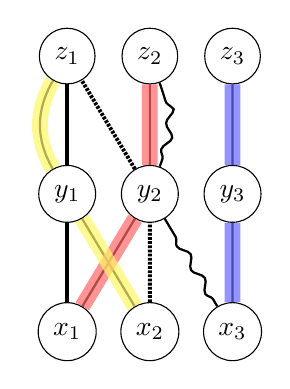
\begin{tikzpicture}[scale=0.7, transform shape = false, rotate=90]
        \pgfkeys{/nodeType/.style={circle, draw},
        /edgeType1/.style={solid, thick, line width=.5mm},
        /edgeType2/.style={solid, thick},
        /edgeType3/.style={thick, decorate, decoration={snake, amplitude=.5mm,pre=lineto,pre length=3pt,post=lineto,post length=3pt}},
        /edgeType4/.style={line width=2mm, draw opacity=0.7}} %highlights the edges of the solution
    
        \def\n{3}
        %n triples (x_i, y_j, z_k) of vertices
        \foreach \i in {1, ..., \n}{
            \node[/nodeType] (x\i) at (0, -1.5*\i) {$x_\i$}; 
            \node[/nodeType] (y\i) at (2.5, -1.5*\i) {$y_\i$}; 
            \node[/nodeType] (z\i) at (5, -1.5*\i) {$z_\i$};
        }
    
        %Edges
        \draw[/edgeType1] (x1) -- (y1) -- (z1);
        \draw[/edgeType2] (x1) -- (y2) -- (z2);
        \draw[/edgeType2] (x2) -- (y1) to[bend left=30] (z1);
        \draw[/edgeType1] [dotted, dash pattern=on 1pt off .5pt] (x2) -- (y2) -- (z1);
        \draw[/edgeType3] (x3) -- (y2);
        \draw[/edgeType3] (y2) to[bend right=20](z2);
        \draw[/edgeType2] (x3) -- (y3) -- (z3);
    
        %Solution
         \draw[/edgeType4] [red!60] (x1) -- (y2) -- (z2);
         \draw[/edgeType4] [yellow!60] (x2) -- (y1) to[bend left=30] (z1);
         \draw[/edgeType4] [blue!60] (x3) -- (y3) -- (z3);    
    \end{tikzpicture}
}
\caption{A \TDMT{} input instance}
\label{fig:sample3dm3}
\end{subfigure}
\quad
\begin{subfigure}[b]{0.58\textwidth}
\centering
\begin{tikzpicture}[scale=0.85, transform shape = false, rotate=90]
    \pgfkeys{/edgeType1/.style={solid, thick, line width=.5mm},
    /edgeType2/.style={solid, thick},
    /edgeType3/.style={thick, decorate, decoration={snake, amplitude=.5mm,pre=lineto,pre length=5pt,post=lineto,post length=5pt}},
    /edgeType4/.style={line width=2mm, green!60, draw opacity=0.7}} %highlights the edges of the solution

    %All vertices
    \node[circle, draw] (x1) at (-1.0, -1.25) {$x_1$};
    \node[circle, draw] (z1) at (4-0.5, -1.25) {$z_1$};
    \setVi{1}{0}{0}{2}
    \node[circle, draw] (x2) at (-1.0, -4.25) {$x_2$};
    \node[circle, draw] (z2) at (4-0.5, -4.25) {$z_2$};
    \setVi{2}{0}{-2.85}{3}
    \node[circle, draw] (x3) at (-1.0, -7.3) {$x_3$};
    \node[circle, draw] (z3) at (4-0.5, -7.3) {$z_3$};
    \setVi{3}{0}{-6.8}{1}

    %Edges
    \draw[/edgeType1] (x1) -- (y111);
    \draw[/edgeType1] (y112) -- (z1);
    \draw[/edgeType2] (y111) -- (y112);
    \draw[/edgeType2] (x2) -- (y121) -- (y122) -- (z1);
    \draw[/edgeType2] (x1) -- (y211) -- (y212) -- (z2);
    \draw[/edgeType1] [dotted, dash pattern=on 1pt off .5pt] (x2) -- (y221);
    \draw[/edgeType2] (y221) -- (y222);
    \draw[/edgeType1] [dotted, dash pattern=on 1pt off .5pt] (y222) -- (z1);
    \draw[/edgeType3] (x3) -- (y231);
    \draw[/edgeType2] (y231) -- (y232);
    \draw[/edgeType3] (y232) -- (z2);
    \draw[/edgeType2] (x3) -- (y311) -- (y312) -- (z3);

    %Solution
    \draw[/edgeType4] [red!60] (x1) -- (y211);
    \draw[/edgeType4] [red!60] (y212) -- (z2);
    \draw[/edgeType4] (y221) -- (y222);
    \draw[/edgeType4] (y231) -- (y232);
    \draw[/edgeType4] [yellow!60] (x2) -- (y121);
    \draw[/edgeType4] [yellow!60] (y122) -- (z1);
    \draw[/edgeType4] (y111) -- (y112);
    \draw[/edgeType4] [blue!60] (x3) -- (y311);
    \draw[/edgeType4] [blue!60] (y312) -- (z3);
\end{tikzpicture}
\caption{The corresponding \GRC{} instance}
\label{fig:sampleGRC}
\end{subfigure}
    \caption{
    A \TDMT{} instance example where $T=\{(x_1, y_1, z_1), (x_1, y_2, z_2),\\ (x_2, y_1, z_1), (x_2, y_2, z_1), (x_3, y_2, z_2), (x_3, y_3, z_3)\}$. Distinct edge types are assigned to each triple, with a solution highlighted.
    The right image depicts the possibility graph of the reduced \GRC{} instance, with a feasible realization highlighted.
    }
    \label{fig:3dm3red}
    \vspace{-.5cm}
\end{figure}

% =>
If a feasible matching $M \subseteq T$ exists in the \TDMT{} instance, we can map it directly to the edges of a valid realization $G$ for the constructed \GRC{} instance.
%
For each $(x_{i_u}, y_j, z_{k_u}) \in M$, using the $u$th occurrence of $y_j$, we add the edges $x_{i_u} y^j_{u,a}$ and $y^j_{u,b} z_{k_u}$ to $G$. For each $(x_{i_v}, y_j, z_{k_v}) \in T \setminus M$, we add the edge $y^j_{v,a} y^j_{v,b}$.
%
Since $M$ is a solution, each vertex in $X \cup Z$ has degree one, satisfying the degree constraints.
%
Additionally, within each group $V_j$, exactly two vertices—$y^j_{u,a}$ and $y^j_{u,b}$ from a triple in $M$—connect to vertices in $X$ and $Z$, respectively. All other vertices within $V_j$ correspond to triples not included in $M$, forming a matching within $V_j$.
%
Therefore, $G$ fulfills both the degree sequence \texttt{d} by assigning degree one to every vertex and the cut list $\mathcal{L}$, meeting all the required constraints for a valid realization.

% <=
Conversely, if a graph $G$ exists that realizes both the degree sequence \texttt{d} and the cut list $\call$, we can construct a feasible matching $M \subseteq T$ for the \TDMT{} instance.
%
Since \texttt{d} specifies a degree of one for each vertex, the edges of $G$ form a matching.
%
Additionally, exactly two vertices within each group $V_j$ are matched to vertices of $X\cup Z$, meaning the remaining vertices within each $V_j$ form an internal matching.
%
These two externally matched vertices must correspond to the same triple in $T$; otherwise, the remaining vertices in $V_j$ could not be paired and meet the type $(V_j, 2)$ cut constraint.
%
Let $M$ consist of the triples in $T$ for which the associated $y^j_{u,a}$ and $y^j_{u,b}$ vertices in $V_j$ are connected to vertices in $X$ and $Z$, respectively.
%
Thus, by construction, vertex $x_i$ connects to $y^j_{u,a}$ and $y^j_{u,b}$ to $z_k$ if and only if the triple $(x_i, y_j, z_k)$ of $T$ belongs to $M$.
%
So $M$ contains exactly one triple per $V_j$, covering each element of $Y$ exactly once, thus $|M| = n$.
%
Since $G$ realizes $\call$, no edges exist between vertices in $X$ and $Z$. Hence, given that $G$ is a matching, each vertex in $X$ connects to exactly one vertex in $Y_a$, and each vertex in $Z$ connects to exactly one vertex in $Y_b$.
%
Consequently, $M$ constitutes a valid matching for the \TDMT{} instance.
\qed
\end{proof}



\section{Final Remarks}
\label{sec:final_remarks}
%resumo do que fizemos
We introduced the \textsc{Graph Realization with Cut Constraints} problem in this work. %, a generalization of the \GRfull{} problem.
%
This problem is interesting because it combines different graph theory concepts, including degree sequence, cut constraints, $f$-factors, and graph realization.
%
We provide a detailed characterization of its computational complexity based on the size of the cuts.
%
Our results show that the problem can be solved in polynomial time when the cuts are small enough (size at most three). However, the complexity significantly increases when the cuts are larger, and we proved that it becomes \classNPH{}.
%
An interesting direction for future work is identifying other graph classes where the possibility graph $\calg$ of a \GRC{} instance ensures polynomial-time solvability. For example, the idea of \cref{prep:tree_graph} might extend to cactus or, more generally, to graphs with bounded degeneracy or treewidth. The case of a planar possibility graph also deserves further investigation. 
%
We also ask about the complexity of {1-in-3 SAT}$_{(2,2)}$, the variant of {1-in-3 SAT} where each variable occurs exactly four times, twice positive and twice negative. 


\begin{credits}
\subsubsection{\ackname}
This work was started during the 6th edition of WoPOCA, which took place in Campinas, São Paulo, Brazil. We thank the organizers and the agencies CNPq (process number 404315/2023-2) and FAEPEX (process number 2422/23).
%
We thank Esther Arkin, Soumya Banerjee, Rezaul Alam Chowdhury, Mayank Goswami, Dominik Kempa, Joseph Mitchell, Valentin Polishchuk, and Steven Skiena for some discussions prior the event, which helped motivate this work.
%
This research has received funding from Rio de Janeiro Research Support Foundation (FAPERJ) under grant agreement E-26/201.344/2021, the National Council for Scientific and Technological Development (CNPq) under grant agreements 309832/2020-9 and \mbox{163645/2021-3}, the São Paulo Research Foundation (FAPESP) under grant agreement 2022/13435-4, and the Brazilian Federal Agency for Support and Evaluation (CAPES) with process numbers 88887.646008/2021-00 and 88887.647870/2021-00. 

\subsubsection{\discintname}
The authors have no competing interests to declare that are
relevant to the content of this article.
\end{credits}

%
% ---- Bibliography ----
%
% BibTeX users should specify bibliography style 'splncs04'.
% References will then be sorted and formatted in the correct style.
%
\bibliographystyle{splncs04}
\bibliography{references}

\end{document}
